% small.tex

\documentclass{beamer}
\usepackage{graphicx}
\renewcommand{\vec}[1]{\mathbf{#1}}
\graphicspath{./images/}
\usetheme{Copenhagen}

\title{Shallow-transfer rule-based machine translation for the Western group of South Slavic languages}
\author{
	Hrvoje Peradin, Filip Petkovski and Francis Tyers
}

\date{May 27, 2014}
\begin{document}
% --------------------------- Title Page --------$------------------ %
\begin{frame}
  \titlepage
\end{frame}
% --------------------------- Slide 2 -------------------------- %
\begin{frame}{Introduction}

\begin{center}
	\begin{figure}
	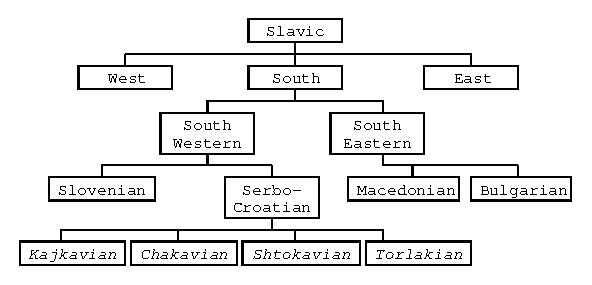
\includegraphics[width=0.8\textwidth]{images/chart.eps}
	\label{fig:1}
	\caption{A traditional division of the South-Slavic languages. All four standard varieties of Serbo-Croatian (Bosnian, Croatian,
Montenegrin, and Serbian) are based on the shtokavian dialect.}
	\end{figure}
\end{center}
\end{frame}

% --------------------------- Slide 3 -------------------------- %
\begin{frame}{The Apertium platform}

The Apertium platform is a modular machine translation system.
The core setup consists of:
\begin{itemize}
\item A letter transducer morphological lexicon
\item Morphological disambiguation module
\item Lexical selection module
\item Syntactic transfer module
\item A letter transducer generator
\end{itemize}
\end{frame}

% --------------------------- Slide 4 -------------------------- %
\begin{frame}{Resources}
Several resources were used extensively throughout the development process:
\begin{itemize}
\item On the Serbo-Croatian side we used the Croatian Language Portal (Hrvatski jezi\v{c}ni portal)
\item The Amebis Besana flective lexicon and other resources were used for the Slovenian side
\item EUDict was used for the bilingual dictionary as the main resource

\end{itemize}
\end{frame}


% --------------------------- Slide 5 -------------------------- %
\begin{frame}{Morphological analysis and generation}
\begin{itemize}

\item The basis for this language pair are the morphological lexicons for Serbo-Croatian and Slovenian developed during Google Summer of Code 2011
\item The Serbo-Croatian dictionary was developed as part of a Serbo-Croatian--Macedonian pair
\item The Slovenian dictionary was developed within a Slovenian--Spanish project
\item Both lexicons had to be synchronized and trimmed down since they were developed with different tagsets and frequency lists 

\end{itemize}
\end{frame}

% --------------------------- Slide 6 -------------------------- %
\begin{frame}{Disambiguation}
\begin{itemize}

\item No freely available tools for disambiguation existed at the time when the project was being developed
\item Satisfactory results were not obtained with the cannonical statistical tagger used in Apertium language pairs
\item We relied solely on Constraint Grammar, which chooses the first output analysis in the case of remaining ambiguity
\item Many of the rules developed earlier for Serbo--Croatian were reused for Slovenian

\end{itemize}
\end{frame}

% --------------------------- Slide 6 -------------------------- %
\begin{frame}{Lexical transfer}
\begin{itemize}

\item Lexical transfer was done using an \emph{lttoolbox} letter transducer and a bilingual dictionary.
\item Additional paradigms were added for simple tagset mismatches which could be easily resolved in this stage
\begin{itemize}
	\item One example are cases when the adjective on one side is synthetic, and on the other analytic (\emph{zdravije} vs \emph{bolj zdravo})
\end{itemize}
\end{itemize}
\end{frame}

% --------------------------- Slide 7 -------------------------- %
\begin{frame}{Lexical selection}
\begin{itemize}
\item Due to a lack of a parallel corpus, Lexical selection was done based on hand-written rules
\item For cases not covered by our hand-written rules, the default translation from the bilingual dictionary was chosen
\item The lexical selection module was used mainly for:
\begin{itemize}
	\item Phonetics-based lexical selection: words that differe in a single phoneme, like \emph{to\v{c}no} and \emph{ta\v{c}no} (accurate)
	\item Croatian months have Slavic-derived names and differ from the original Latin names (\emph{sije\v{c}anj} -- January)
\end{itemize}
\end{itemize}
\end{frame}
\end{document}
